\documentclass[12pt]{article}
\usepackage[utf8]{inputenc}
\title{\vspace{-2.75cm}On Government Borrowing Behavior\vspace{-0.5cm}}
\author{Nicholas Ray}
\date{\vspace{-0.30cm}December 7 2022\vspace{-1cm}}
\usepackage[margin=1in]{geometry}
\usepackage{mathtools,amssymb,amsthm}
\usepackage{setspace}
\usepackage{tikz}
\usepackage{sgame}
\doublespacing
\usepackage[colorlinks,citecolor=cyan,urlcolor=blue,bookmarks=false,hypertexnames=true]{hyperref}
\usepackage[backend=biber, style=authoryear, maxbibnames=99, uniquelist=false]{biblatex}
\renewbibmacro{in:}{}
\renewbibmacro*{volume+number+eid}{%
  \printfield{volume}
  \setunit*{\addnbthinspace}
  \printfield{number}
  \setunit{\addcomma\space}
  \printfield{eid}}
\DeclareFieldFormat[article]{number}{\mkbibparens{#1}}
\AtEveryBibitem{
  \clearfield{issn}
  \clearfield{month}
  \clearfield{urlyear}
  \clearlist{language}
  \clearfield{note}
  \ifentrytype{online}{}{
    \clearfield{url}
  }
}
\DeclareCiteCommand{\citeyear}
    {\usebibmacro{prenote}}
    {\bibhyperref{\printfield{year}}\bibhyperref{\printfield{extrayear}}}
    {\multicitedelim}
    {\usebibmacro{postnote}}
\DeclareCiteCommand{\citeyearpar}[\mkbibparens]
    {\usebibmacro{prenote}}
    {\bibhyperref{\printfield{year}}\bibhyperref{\printfield{extrayear}}}
    {\multicitedelim}
    {\usebibmacro{postnote}}
\addbibresource{ForeignAid.bib}
\begin{document}
\maketitle
\begin{abstract}
    
\end{abstract}

\textit{Keywords}: 

\section*{Introduction}
Since engaging in a ``going out'' strategy around the turn of the century, the People's Republic of China (China) has successfully become the ``lender of first resort'' for developing countries \parencite[1]{dreher2022}.\footnote{All R code, data, and \LaTeX \;code underlying my analysis can be found in the corresponding repository on GitHub at https://github.com/nnray.} There has been an abundance of scholarly work attempting to understand the potential effects of China's contemporary prominence in the global finance arena. Much of this literature focuses on how the international financing behavior of more traditional, Western donors have been affected (e.g., \cite{humphrey2019}; \cite{kilama2016a}) or how the effectiveness of their money has changed (e.g., \cite{blair2022}; \cite{gehring2022}).

Little of this work, however, has looked at how the behavior of recipients of international finance has updated since the availability of Chinese money. This lack of attention is despite recent work that implies that recipient countries may extract benefits from their loan choices in a more Chinese global finance environment. While the literature suggests that recipients stand to gain from receiving both Chinese and Western finance and the subsequently more competitive terms, observations of borrowing practices in Africa do not seemingly reflect that recipients are engaging in a strategy to leverage competition between lenders.
% i.e., that countries take relatively similar levels of both loan types. 

I argue that this is due to time-inconsistency problems where countries prefer Western or Chinese loans over the other in the short-run. Understanding the debt composition of developing countries is an increasingly important issue as public debt continues to rise. This research could also shed light on literature concerned about China's interaction with the liberal international order (LIO) and spark a new research agenda studying recipient behavior. \textbf{more about contributions}

\textbf{layout of the paper}

\section*{What Demands Explanation and Why}
There is evidence that African countries are offered fewer loan conditions from the World Bank (\cite{hernandez2017}) and that Western aid is less sensitive to policy and institutional quality (\cite{annen2021}) when they are recipients of Chinese finance. Although Dreher et al. \citeyear{dreher2021} did not find that the effectiveness of aid from the United States (U.S.) is negatively affected by the presence of Chinese aid, their results do suggest that U.S. aid effectiveness increases in the absence of Chinese aid. In sum, this evidence intimates that Western entities are changing their international financial behavior in response to China in a way that benefits recipients.

There is also tentative evidence that China reciprocates these actions. Dreher et al. \citeyear{dreher2018} find that Chinese finance increases with Western development assistance, which they interpret as competitive behavior from China. Taken together, the literature seems to imply that there is some financial competition between the West and China that recipients may be able to take advantage of to procure more favorable borrowing terms. If recipients value better loan terms, including lower conditionality, and are willing to take on more debt, it follows that they should be attempting to stimulate this competition by diversifying their loan diet to include both Western and Chinese debt. While this logic stemming from the literature does not stipulate an exact proportion of Western finance to Chinese finance that optimizes recipient benefits, it should not be the case that countries borrow exclusively from one or the other. Interrogatively, do African countries at the center of this seeming financial competition borrow from the West and China at similar rates to benefit from their competition? 

A cursory view of African debt suggests that this is not universally the case. The proportion of Chinese loans to Western loans varies substantially between counties and further that some countries almost entirely borrow from either China or the West when taking money from governments. For example, compare table 1 and table 2, which show the estimated composition of public debt in Cabo Verde and Djibouti, respectively (\cite{jubileedebtcampaign2018}). Cabo Verde owes only 1\% of its estimated total debt to China while debt to Portugal and other unspecified countries exceeds 25\%. In Djibouti, meanwhile, 68\% of its estimated debt can be attributed to China.

\begin{table}
    \centering
    \includegraphics[scale=0.5]{Figures/CaboVerde.png}
    \caption{Estimated Debt for Cabo Verde}
    \vspace{1cm}
    \includegraphics[scale=0.5025]{Figures/Djibouti.png}
    \caption{Estimated Debt for Djibouti}
\end{table}

Thus, the variance in debt composition and the seeming failure of countries to borrow in a more equal manner between China and Western entities must be explained. In other words, how do recipient countries decide between taking loans from China and the West? Taking loans is costly, at least in the long-run, and recipients presumably want to maximize the payoff they receive from borrowing. Related literature seems to not have fully considered recipient decision-making with regard to choosing a borrower, instead largely focusing on macroeconomic and political determinants of government debt (e.g., \cite{bittencourt2015} ; \cite{swamy2015}) or the determinants of lender behavior (e.g., \cite{dreher2018}).

\begin{table}
    \centering
    \includegraphics[scale=0.53]{Figures/summary1.png}
    \caption{Summary Table of Debt and Loans in Africa}
\end{table}

\section*{My Explanation}
I argue that the variation observed in African borrowing practices is a result of strategic considerations on behalf of recipients. Specifically, I argue that some countries take Chinese and Western finance at substantially different rates due to dissimilarities in the conditions of Western and Chinese loans and the subsequent evaluations of loan value by recipients.

There is evidence that China might be simultaneously more strict on the economic conditions on their finance (e.g., \cite{dreher2018}) while also less strict on the political conditions imposed (e.g., \cite{dreher2018}). Western loans, by contrast, seem more politically strict than economic (\cite{hernandez2017}). This dissimilarity leads to time-inconsistency problems, where in the short-term countries prefer either less severe economic or political conditions instead of minimizing the joint conditionality over the long-term.

%going back to the motivating example of Cabo Verde and Djibouti, these examples indeed fit this story as Cabo Verde is much more ``free'' than Djibouti, at least according to Freedom House

One implication is that more democratic countries should be more sensitive to explicitly political conditions and, thus, prefer Western loans $ceteris\;paribus$. This could also explain Dreher et al.'s (\citeyear{dreher2018}) findings that Chinese loans seem to flow to more corrupt countries and those with poorer political institutions.

\subsubsection*{Figure 1: Non-Democratic Country Loan Preference, $ceteris\;paribus$}
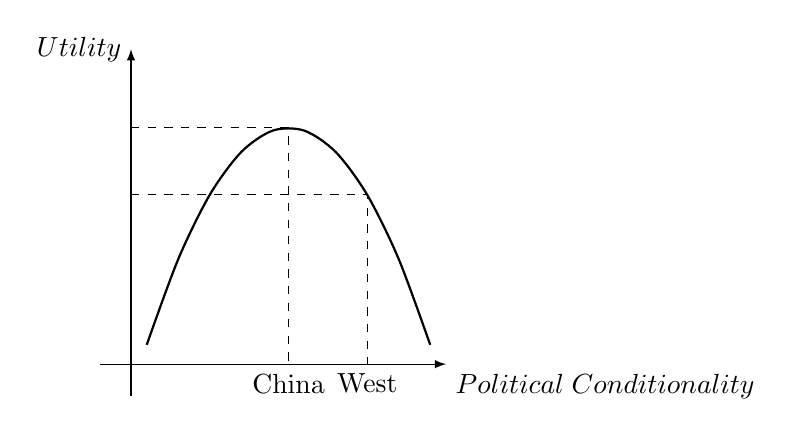
\begin{tikzpicture}[scale=2,declare function={F(\x) = 1.7*(2*\x-\x*\x)-0.2;}]
  \draw[-latex] (0,-0.2) -- (0,2) node[left]{$Utility$};
  \draw[-latex] (-0.2,0) -- (2,0) node[below right]{$Political\;Conditionality$};
  \draw[domain=0.1:1.9,samples=10,smooth,thick] plot (\x, {F(\x)}); 
  \coordinate (max) at (0,{F(1)});
  \draw[dashed] (max) -| (1,0) node[pos=1,below]{China};
  \coordinate (max) at (0,{F(1.5)});
  \draw[dashed] (max) -| (1.5,0) node[pos=1,below]{West};
\end{tikzpicture}

\section*{Research Design}
The implication above leads to the following hypotheses:
\begin{align*}
    H_{1a}&:\;\text{Democracies should receive more Western loans than Chinese loans}\\
    H_{1b}&:\;\text{Non-democracies should receive more Chinese loans than Western loans}\\
\end{align*}
To test these hypotheses I intend to focus on the international loan environment in Africa since from the years 2000 to 2020 due the continent being a major area of focus for China's finance projects and this being the time period most relevant for Chinese finance. I will fit a logit/probit model with the lender type (e.g., majority Western or not) as my dependent variable. The main explanatory variables will be regime type and a measure for loan conditionality. Ideally, an instrumental variable will be used for regime type since there is theoretically expected to be simultaneity present. Further, I will include gross domestic product (GDP) per capita as a control for recipient need and an additional control for the gross sum of the loan to ensure comparison.

I plan to use data from William \& Mary's ``Aiddata'' lab for Chinese loans (\cite{custer2021}) and data from the Organization for Economic Co-operation and Development (OECD) on Western loans (\cite{organizationforeconomicco-operationanddevelopment2022a}). GDP per capita stems from the United Nations (\cite{unitednationsstatisticsdivision2019}). For regime type, I intend to use an updated version of Cheibub et al.'s dictatorship and democracy index (\cite{cheibub2010}).

\section*{Preliminary Analysis}

\begin{table}
    \centering
    \includegraphics[scale=0.53]{Figures/summary2.png}
    \caption{Summary Table of Variables}
\end{table}

\begin{table}
    \centering
    \includegraphics[scale=0.53]{Figures/summary3.png}
    \caption{Summary Table of Variables}
\end{table}


\begin{table}[!htbp] \centering 
  \caption{Accounting for Variation in the Ratio between Chinese and World Bank Loans} 
  \label{} 
\begin{tabular}{@{\extracolsep{5pt}}lc} 
\\[-1.8ex]\hline 
\hline \\[-1.8ex] 
 & \multicolumn{1}{c}{\textit{Dependent variable:}} \\ 
\cline{2-2} 
\\[-1.8ex] & Ratio (China/World Bank) \\ 
\hline \\[-1.8ex] 
 GDP per capita & $-$0.030$^{***}$ \\ 
  & (0.007) \\ 
  & \\ 
 Polity & $-$1.379 \\ 
  & (4.243) \\ 
  & \\ 
\hline \\[-1.8ex] 
Observations & 874 \\ 
R$^{2}$ & 0.024 \\ 
Adjusted R$^{2}$ & $-$0.059 \\ 
F Statistic & 9.792$^{***}$ (df = 2; 805) \\ 
\hline 
\hline \\[-1.8ex] 
\textit{Note:}  & \multicolumn{1}{r}{$^{*}$p$<$0.1; $^{**}$p$<$0.05; $^{***}$p$<$0.01} \\ 
\end{tabular} 
\end{table} 

\section*{Discussion and Conclusion}


\nocite{curini2020}
\pagebreak
\printbibliography
\end{document}